% LAB 6: File I/O
% 
% CSE/IT 107: Introduction to Programming
% New Mexico Tech
% 
% Prepared by Russell White and Christopher Koch
% Spring 2015
\documentclass[11pt]{cselabheader}

%%%%%%%%%%%%%%%%%% SET TITLES %%%%%%%%%%%%%%%%%%%%%%%%%
\fancyhead[R]{Lab 6: File I/O}
\title{Lab 6: File I/O}

\begin{document}

\maketitle

\pagenumbering{roman}
\hrule
\begin{quotation}
``The danger that computers will become like humans is not as big as the danger
that humans will become like computers.'' (``Die Gefahr, dass der Computer so
wird wie der Mensch ist nicht so gro\ss, wie die Gefahr, dass der Mensch so wird
wie der Computer.'')
\end{quotation}
\begin{flushright}
--- Konrad Zuse
\end{flushright}

\begin{quotation}
``First, solve the problem. Then, write the code.''
\end{quotation}
\begin{flushright}
--- John Johnson
\end{flushright}

\begin{quotation}
``I don’t need to waste my time with a computer just because I am a computer
scientist.''
\end{quotation}
\begin{flushright}
--- Edsger W. Dijkstra
\end{flushright}

\hrule

\section*{Introduction}
\addcontentsline{toc}{section}{Introduction}

In previous labs, we taught you how to use functions, math, lists, strings, and
the like. We will combine all that in this lab and teach you how to interact
with files. This will lead us to do some exciting data analysis!

\pagebreak

\tableofcontents

\pagebreak
\pagenumbering{arabic}
\section{File I/O}
Knowing how to work with files is important, since it lets us store and retrieve
data beyond the scope of the single execution of a program. To open a file for
reading or writing we will use the \pythoninline!open()! function. The following
example opens a file and writes ``Hello World'' to it.

\begin{python3code}
output_file = open("hello.txt", "w")

print("Hello World", file=output_file)
output_file.close()
\end{python3code}

Files can also be written to by using \pythoninline!.write(contents)!. This
method will write only the characters given to it, so a newline \lstinline{\\n}
must be included for a newline.

\begin{python3code}
output_file = open("hello.txt", "w")

output_file.write("Hello World\n")
output_file.close()
\end{python3code}

The arguments to the \pythoninline!open()! function are, in order, the name of
the file to open and the mode in which to open the file. ``w'' means that the
file is to be opened in write mode. If the file does not exist, this will create
the file. If it does exist, then the contents of the file will be cleared in
preparation for the new ones.

Other options include ``a'', which is similar to ``w'' but will not clear the
contents of an existing file and will instead append the new data to the end,
and ``r'' which will read the file instead. If ``r'' is used and the file does
not exist, then an error will occur. The following code takes a filename as user
input, then prints out the entire contents of that file.

\begin{table}[!ht]
  \centering
  \begin{tabular}{ll}
    Mode & What it does \\
    \midrule
    a & Create file if does not exist, open file, append contents to the end \\
    w & Create file if does not exist, open file, write contents to the beginning
    of file \\
    r & Open file, permit reading only \\
  \end{tabular}
\end{table}

\begin{python3code}
filename = input("What file should be read? ")

input_file = open(filename, "r")
for line in input_file:
    print(line, end="")

input_file.close()
\end{python3code}

The additional concepts introduced in these examples are:

\begin{itemize}
\item The \pythoninline!print()! function can have an additional ``file'' parameter
  passed to it to allow writing to a file. This causes it to send its output to
  the file rather than the screen, though otherwise it performs identically.

\item The \pythoninline!print()! function has an additional optional ``end''
  parameter. This allows you to specify what should be printed after the main
  string given to it. This is important because it defaults to \pythoninline!"\n"!,
  which causes a newline after every print statement. By changing ``end'' to
  \pythoninline!""! we prevent a newline from being added after every line of the
  file is printed. This is because each line in the file already has a newline
  at the end of it, so we don't need \pythoninline!print()! to add its own.

\item \pythoninline!.close()! is used to properly tell Python that you are done
  with a file and close your connection to it. This isn't \emph{strictly}
  required, but without it you risk the file being corrupted or other programs
  being unable to access that file.

\item When reading from a file, Python can use a \pythoninline!for! loop to go
  through each line in sequence. This works identically to if you think of the
  file as a list with every line being a different element of the list. The
  entirety of the file can also be read into a single string using the
  \pythoninline!.read()! function.

\begin{pyconcode}
>>> input_file = open("test.py", "r")
>>> contents = input_file.read()
>>> print(contents)
filename = input("What file should be read? ")

input_file = open(filename, "r")
for line in input_file:
    print(line, end="")

input_file.close()
\end{pyconcode}

\item \pythoninline!.readlines()! can be used to read all of a file at once, though
  it splits the file into a list. Each element of the list will be one line of
  the file being read.
\end{itemize}

\subsection{Files Using \protect\pythoninline!with!}
\label{sec:with}

Since every file that you open should be closed after use, Python has an easy
way to do this for you. Using the \pythoninline!with! command, your file will
automatically be closed when the \pythoninline!with! block finished executing.

\begin{python3code}
filename = input("Enter filename: ")

with open(filename, "r") as file:
    for line in file:
        print(line, end="")
# file.close() is not necessary, because "with" closed it for us
\end{python3code}

\begin{warningbox}{Using \protect\pythoninline!with!}
  Always use the \pythoninline!with! statement to deal with file I/O in Python.
\end{warningbox}

\pagebreak
\section{Exceptions}

An \emph{exception} is an error message in Python. When a certain operation
encounters an error, it can \emph{raise} an exception that is then passed on to
the user:

\begin{pyconcode}
>>> 43 / 0
Traceback (most recent call last):
  File "<input>", line 1, in <module>
ZeroDivisionError: division by zero
\end{pyconcode}

However, in a lot of cases you may want to handle an exception as a developer
and not have it displayed to the user. This is where the \pythoninline!try! and
\pythoninline!except! statements come in.

When working with input and output it is important to check for exceptions.  
\begin{itemize}
  \item For example, when we try to open a file that does not exist we'd like to
    exit the program safely or recover rather than observing the unexpected
    results.
  \item Exception handling in python consists of "try-except" blocks.  In a
    "try-except" block we execute instructions in the \pythoninline!try! block
    and catch errors in one or more following \pythoninline!except! blocks.  
  \item The \pythoninline!except! block is only executed if an exception is
    caught in the \pythoninline!try! block.
  \item Additionally, when an error is
    caught in the \pythoninline!try! block we stop executing commands in the
    \pythoninline!try!  block and jump to the first \pythoninline!except! or
    optional \pythoninline!finally! block.
\end{itemize}

The following example throws a division by zero error and prints ``division by
zero'':

\begin{python3code}
prime = 7

try:
    result = prime / 0
    result = 7*42
except ZeroDivisionError as err:
    print(err)
\end{python3code}

Looking at the code above, since the error is thrown on line 5, line 6 is never
executed.

If you are experimenting with code and want to know the name of an exception
that is thrown, take a look at the error message:

\begin{pyconcode}
>>> float('obviously not convertable')
Traceback (most recent call last):
  File "<input>", line 1, in <module>
ValueError: could not convert string to float: 'obviously not convertable'
\end{pyconcode}

The part highlighted in red here is the name of the error message,
\pythoninline!ValueErrror!.

Hence, if you are getting user input and want to check whether it is the correct
type, use a try-except block around the conversion:

\begin{python3code}
try:
    x = int(input('Enter an integer number: '))
except ValueError:
    print('You did not enter an integer!')
else:
    print('You entered {}'.format(x))
\end{python3code}

Notice that you can use an \pythoninline!else! block to be executed if no
exception was thrown.

Any \pythoninline!except!  block that does not list built-in
exceptions will catch all exceptions not listed in previous
\pythoninline!except! blocks.  For example, the following code will throw an
error if the user enters anything but an integer:

\begin{python3code}
try:
    x = int(input("Enter a number: "))
except:
    print("Unknown error.")
    raise
else:
    print("You entered: " + str(x))
\end{python3code}

The \pythoninline!raise! keyword causes a stack trace and prints out additional
information if an exception is encountered.  The \pythoninline!else! block is
always optional and will always be executed if no exceptions are thrown in the
\pythoninline!try! block.  There are many more built-in exceptions such as
\pythoninline!IOError! that can be found here:

\begin{center}
\url{https://docs.python.org/3.2/library/exceptions.html}
\end{center}

If you try to open a file that does not exist for reading, Python will display
an error message:

\begin{pyconcode}
>>> open("not_a_file.txt", "r")
Traceback (most recent call last):
  File "<stdin>", line 1, in <module>
FileNotFoundError: [Errno 2] No such file or directory: 'not_a_file.txt'
\end{pyconcode}

In this case, the error is \pythoninline!FileNotFoundError!. Normally having an
error occur will end your program, but we can use \pythoninline!try-except! in
order to perform a special action in case of an error.

\begin{itemize}
  \item The \pythoninline!finally! block is where clean-up actions are performed
    and is always executed after leaving the \pythoninline!try! block.
\end{itemize}

The following is a good example of using \pythoninline!with! and exception
handling together.

\begin{python3code}
filename = input('Enter a filename >>> ')

try:
    with open(filename, 'r') as f:
        sum = 0
        for line in f:
            sum += float(line)
except FileNotFoundError:
    print('Filename you entered is wrong')
except ValueError:
    print('The file you entered had a line containing a non-float element.')
else:
    print('Sum of all numbers in file is {}'.format(sum))
finally:
    print('Goodbye.')
\end{python3code}

%\section{Recursion}
\pagebreak
\section{Instantiating Turtles}
Similarly to being able to open multiple files, we can also create multiple
turtles to draw more complex designs. This is done using the
\pythoninline!turtle.Turtle()! function. This function returns a turtle object,
which we can call every other normal turtle function on.

\begin{python3code}
import turtle

first = turtle.Turtle()
second = turtle.Turtle()

first.forward(50)
second.forward(50)
first.left(90)
second.right(90)
first.forward(50)
second.forward(50)
first.right(90)
second.left(90)
first.forward(50)
second.forward(50)
\end{python3code}

\begin{figure}[h]
  \centering
  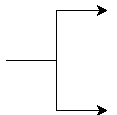
\includegraphics[width=1.0in]{img/turtle_prong}
\end{figure}

If we add a group of turtles to a list, we can easily apply the same commands to all of them, as in this example:

\begin{python3code}
import turtle

turtles = []
first = turtle.Turtle()
first.speed(0)
turtles.append(first)

second = turtle.Turtle()
second.speed(0)
second.right(90)
turtles.append(second)

third = turtle.Turtle()
third.speed(0)
third.right(180)
turtles.append(third)

fourth = turtle.Turtle()
fourth.speed(0)
fourth.right(270)
turtles.append(fourth)

for i in range(200):
    for turt in turtles:
        turt.forward(i/5)
        turt.left(10)
\end{python3code}

\begin{figure}[h]
  \centering
  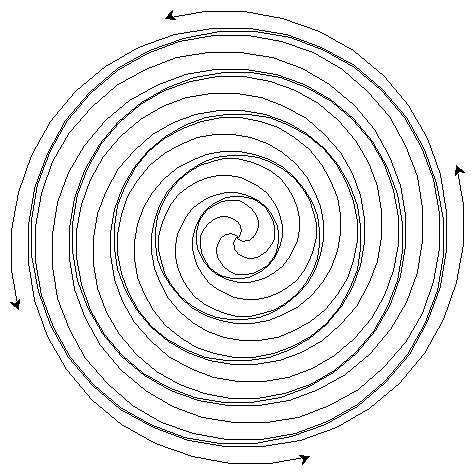
\includegraphics[width=0.6\textwidth]{img/fancy_spiral}
\end{figure}

\pagebreak
\section{Matplotlib}
Matplotlib is a Python library that provides MATLAB-like plotting functions.
Simple plots such as bar graphs and line graphs are very easy to create using
matplotlib.

Using the \pythoninline!.plot()! and \pythoninline!.bar()! methods of
\pythoninline!matplotlib.pyplot!, we can quickly show line and bar graphs.
\pythoninline!.plot()! and \pythoninline!.bar()! take a dataset for x and a
dataset for y, with many more optional parameters such as \pythoninline!align!.
These examples use data from
\begin{center}
  \url{http://nmt.edu/~olegm/382labs/2cities.csv}
\end{center}

\begin{itemize}
  \item Data set is three columns: a data point number, the temperature in
    Tucson, and the temperature in Eugene in degrees Celsius.
\end{itemize}

\begin{figure}[h]
  \centering
  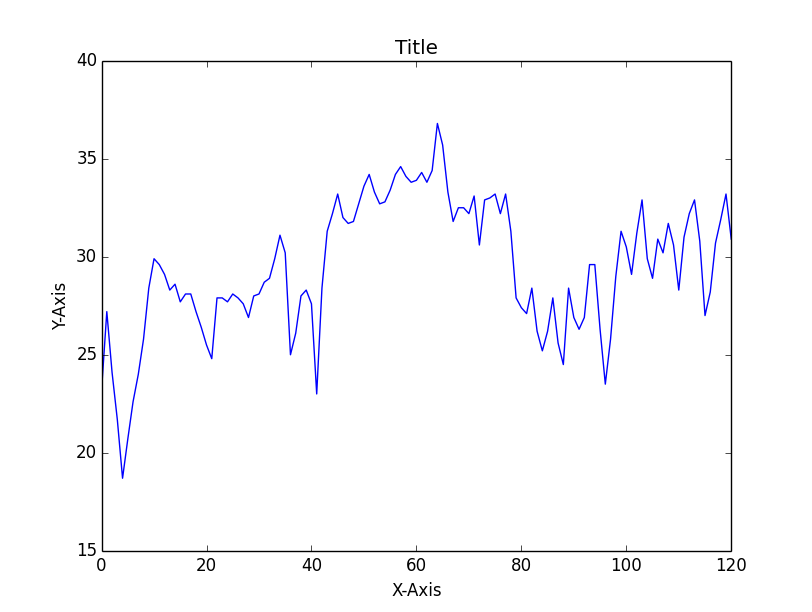
\includegraphics[width=0.85\textwidth]{img/line1.png}
  \caption{Line plot example: temperature data from Tucson, AZ.}
  \label{fig:line1}
\end{figure}

The following code will show a line plot of the dataset. You can see the graph
it produces in Figure~\ref{fig:line1}.

\begin{python3code}
import matplotlib.pyplot as plt

with open("2cities.csv", "r") as f:
    lines = f.readlines()

temps = []
for line in lines:
    cols = line.split()
    try:
        if len(cols) > 1:
            temps.append(float(cols[1]))
    except ValueError:
        pass # could not convert to float, must be first row with headers

plt.plot(list(range(len(temps))), temps)
plt.xlabel("Data point")
plt.ylabel("Temperature in degrees Celsius")
plt.title("Temperature in Tucson, AZ over 120 days")
plt.show()
\end{python3code}

Next, we are trying to create a histogram of the data.

\begin{itemize}
  \item A histogram is a bar graph where a bar represents
    a temperature \emph{range}. We call one of these ranges a bin or a bucket.
  \item 
    For example, the temperatures in Tucson in the data set
    range from 18$^\circ$ Celsius to 37$^\circ$ Celsius. We would create a
    histogram spanning temperatures from $15^\circ$ to $40^\circ$ Celsius with
    bins of size $5^\circ$ Celsius. That means a bin for $15$ to $20$ degrees
    Celsius, a bin for $20$ to $25$ degrees Celsius, etc.
\end{itemize}

\begin{python3code}
import matplotlib.pyplot as plt

with open("2cities.csv", "r") as f:
    lines = f.readlines()

temps = []
for line in lines:
    # columns in 2cities.csv are [data point number, tucson temp, eugene temp]
    cols = line.split()
    try:
        if len(cols) > 1:
            temps.append(float(cols[1]))
    except ValueError:
        pass # could not convert to float, must be first row with headers

numbuckets = 5
binnumbers = range(0, numbuckets)
counts = []
for bucketno in binnumbers:
    bucket = []
    for temp in temps:
        if 15 + bucketno * 5 < temp < 15 + (bucketno + 1) * 5:
            bucket.append(temp)
    # Count how many temperatures are in this bucket.
    # This count will be the height of the bar in the graph.
    counts.append(len(bucket))

xlabels = []
for bucket in binnumbers:
    xlabels.append("{} to {}C".format(15 + bucket * 5, 15 + (bucket + 1) * 5))

plt.bar(binnumbers, counts, align="center")
plt.xticks(binnumbers, xlabels)
plt.xlabel("Temperature in Celsius")
plt.ylabel("Number of times occured")
plt.title("Histogram of Temperatures in Tucson, AZ")
plt.show()
\end{python3code}

This code will produce this output of the input data sorted into 10 bins of size
5 (not showing empty bins) as seen Figure~\ref{fig:bar1}.

\begin{figure}[h]
  \centering
  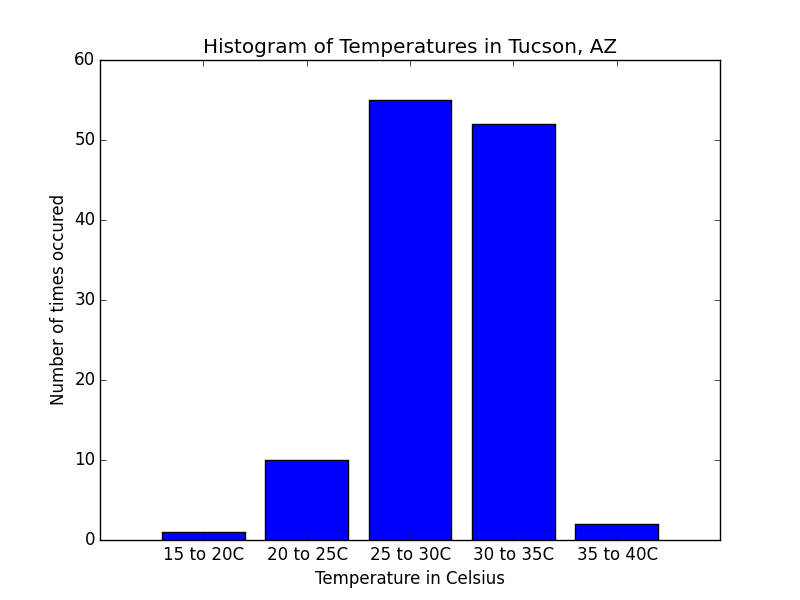
\includegraphics[width=0.85\textwidth]{img/lab6_histo_tucson.png}
  \caption{Input data sorted into 5 bins of size 5$^\circ$ Celsius.}
  \label{fig:bar1}
\end{figure}

\subsection{More Documentation}

\begin{itemize}
  \item \pythoninline!.plot()! function documentation:
    \begin{center}
      \url{http://matplotlib.org/api/pyplot\_api.html#matplotlib.pyplot.plot}
    \end{center}
  \item \pythoninline!.bar()! function documentation:
    \begin{center}
      \url{http://matplotlib.org/api/pyplot\_api.html#matplotlib.pyplot.bar}
    \end{center}
  \item Documentation overview for \pythoninline{matplotlib.pyplot}:
    \begin{center}
      \url{http://matplotlib.org/api/pyplot\_summary.html}
    \end{center}
\end{itemize}

\pagebreak
\section{Exercises}
\label{sec:ex}

\begin{warningbox}{Using \protect\pythoninline!with!}
  Always use the \pythoninline!with! statement to deal with file I/O in Python.
  See Section~\ref{sec:with}.
\end{warningbox}

\begin{ex}[save.py] Write a program that takes in a filename, then takes in
  a series of lines of input until a blank line is entered, writing each line to
  the file with the given name. After the blank line is entered, properly close
  the file before ending the program.
\end{ex}

\begin{ex}[word\_count.py] Write a program that
  takes in a filename and string as input. Then print how many times that string
  appears inside the chosen file. If the file does not exist, continue asking
  for a filename until one is given that exists. Use your source code file as
  test input.
\end{ex}

\begin{ex}[diff.py]
  Write a ``diff'' program that prints out the differences, line by line, of
  two files.  Your program should ask the user for the names of two files,
  then print the differences between them.  Follow the format output as shown
  below. Make sure to use proper error handling techniques for file I/O.

  Example:

  \begin{listing}[H]
    \vspace{-0.5em}
    \begin{verbatimcode}
John goes to work.
Keith and Kyle went to the Ensiferum concert.
Alice ate an apple pie.
Joe cut down a tree.
The dog jumped over the wall.
    \end{verbatimcode}
    \vspace{-0.5em}
    \caption{file1.txt}
    \vspace{-0.5em}
  \end{listing}

  \begin{listing}[H]
    \vspace{-0.5em}
    \begin{verbatimcode}
John goes to work.
Coral went to a Kesha concert.
Alice ate an apple pie.
Joe planted a tree.
The dog jumped over the wall.
    \end{verbatimcode}
    \vspace{-0.5em}
    \caption{file2.txt}
    \vspace{-0.5em}
  \end{listing}

  \begin{verbatimcode}
Enter file name 1 >>> file1.txt
Enter file name 2 >>> file2.txt

2c2
< Keith and Kyle went to the Ensiferum concert.
---
> Coral went to a Kesha concert.
4c4
< Joe cut down a tree.
---
> Joe planted a tree.
  \end{verbatimcode}
\end{ex}


\begin{ex}[navigate3.py] Modify navigate.py so that, rather than take
  instructions from the command line, it reads from a file (specified by user
  input) to determine what the turtle will do. Additionally, you will be adding
  the ``split'' command. This command will use instantiation of new turtles in
  order to draw multiple lines at once. Every new command will apply to every
  turtle that currently exists. The file will have on instruction per line. The
  possible instructions are:

  \begin{description}
    \item[forward X] Move all turtles forward X.
    \item[left X] Turn all turtles X degrees to the left.
    \item[right X] Turn all turtles X degrees to the right.
    \item[split X] Split all turtles into new turtles. Each new turtle will be turned X degrees to the right.
  \end{description}

  In order to properly implement split, you will probably need to look up the
turtle functions \pythoninline!.position()!, \pythoninline!.setposition()!,
  \pythoninline!.setheading()!, \pythoninline!.heading()!, \pythoninline!.penup()!, and
  \pythoninline!.pendown()!. Turtle documentation is available at
  \begin{center}
    \url{https://docs.python.org/3/library/turtle.html}
  \end{center}

  You will also likely use the \pythoninline!.split()! command when getting
  input, which splits a single string into an array around the string's
  spaces.
  \begin{pyconcode}
>>> print("this is a phrase".split())
['this', 'is', 'a', 'phrase']
>>> print("hi,hi,hi".split(",")
['hi', 'hi', 'hi']
  \end{pyconcode}

  \emph{Suggestion:} Split each command into a different function to help keep their logic separate.

  Sample Input File:

  \begin{verbatimcode}
forward 50
left 20
split 40
forward 50
left 20
split 40
forward 50
left 20
split 40
forward 50
left 20
split 40
forward 50
left 20
  \end{verbatimcode}

  Sample Output
  \begin{center}
    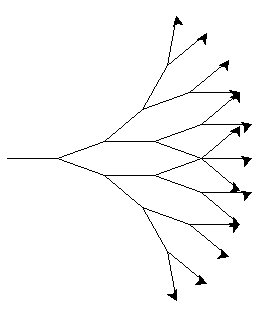
\includegraphics[width=0.4\textwidth]{img/nav3_example}
  \end{center}
\end{ex}
\begin{ex}[testscores.py]
  Download the file \texttt{actsat.txt} provided on Canvas. It contains the
  following data by column:

  \begin{enumerate}[\text{Column} 1~]
    \item 2-letter state/territory code (includes DC)
    \item \% of graduates in that state taking the ACT
    \item Average composite ACT score
    \item \% of graduates in that state taking the SAT
    \item Average SAT Math score
    \item Average SAT Reading score
    \item Average SAT Writing score
  \end{enumerate}

  Each SAT section is out of 800 points, while the ACT is out of 36 points.

  Write a program that generates the following charts:
  \begin{enumerate}
    \item A histogram of average ACT scores with bins of size $1$ between a
      score of $18$ and $24$.
    \item A double bar chart that compares the composite ACT score with the
      total score of all 3 SAT tests for all 51 states/territories.
    \item Produce the same chart as in part 2, but only for states in which
      less than 50\% take the ACT and more than 50\% take the SAT. (There
      should be 21 states/territories like this.)
  \end{enumerate}

  You may have to do some research on the matplotlib website on how to create
  a double bar graph. Take a look at the example code on their website.
  Remember to label your axes and title your graph.
\end{ex}

\section{Submitting}

You should submit your code as a tarball. It should contain all files
used in the exercises for this lab. The submitted file should be named
\begin{center}
  \texttt{cse107\_firstname\_lastname\_lab6.tar.gz}
\end{center}

\begin{center}
  \textbf{Upload your tarball to Canvas.}
\end{center}

\listoftheorems


\end{document}
